\chapter{Fake Tau Estimation Additional Material}
\markboth{}{Appendix A}
%\section{Z+jets selection triggers}
%\label{app:FTTF_Zjets_data_trigs}
%The triggers used to defined the gluon abundant Z boson with associated jets  data region used to derive the \ac{FF} values for the \ac{TFFT} are defined here:
%\begin{itemize}
%\item If 2015 data is use then either of the following triggers are required to be passed
%\begin{itemize}
%\item HLT\_mu20\_iloose\_L1MU15
%\item HLT\_mu50
%\end{itemize}
%\item For data 2016 onwards either of the following triggers are required to be passed instead
%\begin{itemize}
%\item HLT\_mu26\_ivarmedium
%\item HLT\_mu50
%\end{itemize}
%\end{itemize}


%\section{Multi-jet selection triggers}
%\label{app:FTTF_Dijets_data_trigs}
%The triggers used to defined the quark abundant Multi-jet data region used to derive the \ac{FF} values for the \ac{TFFT} are defined here with their corresponding offline \pt\ thresholds:
%\begin{itemize}
%\item HLT\_j15 with offline $\pt\,>\,20$ GeV
%\item HLT\_j25 with offline $\pt\,>\,35$ GeV
%\item HLT\_j35 with offline $\pt\,>\,45$ GeV
%\item HLT\_j85 with offline $\pt\,>\,110$ GeV
%\item HLT\_j110 with offline $\pt\,>\,120$ GeV
%\item HLT\_j175 with offline $\pt\,>\,216$ GeV
%\item HLT\_j260 with offline $\pt\,>\,300$ GeV
%\item HLT\_j360 with offline $\pt\,>\,400$ GeV
%\item HLT\_j400 with offline $\pt\,>\,440$ GeV
%\item HLT\_j420 with offline $\pt\,>\,460$ GeV
%\end{itemize}
%
%\newpage
\section{MC templates}
\label{app:AODtemplates}
In this section the track based jet width distributions derived using the base selection samples described in Section ~\ref{subsec:AODsel} of Chapter ~\ref{ch:fake_est} are shown. The shown distributions have been made using the following selection requirements:
\begin{itemize}
\item[] \htau\ \pt\ > 20 \gev
\item[] \htau\ minimum \ac{BDT} score > 0.05
\item[] \htau\ fails the \textit{Medium} \ac{BDT} working point
\item[] no \ac{JVT} requirement 
\item[] no trigger requirement
\end{itemize}
Diagram have been produced for the full set of available \pt\ bins and for both 1 prong and 3 prong \ftau\ candidates. 

\newpage
\subsection*{2015-2016}
\begin{figure}[H]
	\begin{center}
\subbottom[]{\includegraphics[width=0.35\textwidth]{FakeTau/AOD/MC16a/1p/gluon_Jet_Width_for_All_samples_and_in_bin_[20,30]_for_1_prong.png}}\hspace{0.05\textwidth}
\subbottom[]{\includegraphics[width=0.35\textwidth]{FakeTau/AOD/MC16a/3p/gluon_Jet_Width_for_All_samples_and_in_bin_[20,30]_for_3_prong.png}}\hspace{0.05\textwidth}
\subbottom[]{\includegraphics[width=0.35\textwidth]{FakeTau/AOD/MC16a/3p/gluon_Jet_Width_for_All_samples_and_in_bin_[30,40]_for_3_prong.png}}\hspace{0.05\textwidth}
\subbottom[]{\includegraphics[width=0.35\textwidth]{FakeTau/AOD/MC16a/3p/gluon_Jet_Width_for_All_samples_and_in_bin_[30,40]_for_3_prong.png}}\hspace{0.05\textwidth}
\subbottom[]{\includegraphics[width=0.35\textwidth]{FakeTau/AOD/MC16a/1p/gluon_Jet_Width_for_All_samples_and_in_bin_[40,60]_for_1_prong.png}}\hspace{0.05\textwidth}
\subbottom[]{\includegraphics[width=0.35\textwidth]{FakeTau/AOD/MC16a/3p/gluon_Jet_Width_for_All_samples_and_in_bin_[40,60]_for_3_prong.png}}\hspace{0.05\textwidth}
\subbottom[]{\includegraphics[width=0.35\textwidth]{FakeTau/AOD/MC16a/1p/gluon_Jet_Width_for_All_samples_and_in_bin_[60,90]_for_1_prong.png}}\hspace{0.05\textwidth}
\subbottom[]{\includegraphics[width=0.35\textwidth]{FakeTau/AOD/MC16a/3p/gluon_Jet_Width_for_All_samples_and_in_bin_[60,90]_for_3_prong.png}}\hspace{0.05\textwidth}
\subbottom[]{\includegraphics[width=0.35\textwidth]{FakeTau/AOD/MC16a/1p/gluon_Jet_Width_for_All_samples_and_in_bin_[90,150]_for_1_prong.png}}\hspace{0.05\textwidth}
\subbottom[]{\includegraphics[width=0.35\textwidth]{FakeTau/AOD/MC16a/3p/gluon_Jet_Width_for_All_samples_and_in_bin_[90,150]_for_3_prong.png}}\hspace{0.01\textwidth}
		\end{center}
		\caption{Jet Width templates of gluon tau-faking jets separated into \pt\ bins, going from top as the lowest \pt\ bin to bottom being the highest. Left column shows templates for 1 prong tau, while right columns shows 3 prong tau templates. Samples shown have been produced for the 2015-2016 data collection period pile-up conditions.}
		\label{fig:2016_gluon_templates}
\end{figure}
	
\begin{figure}[H]
	\begin{center}
\subbottom[]{\includegraphics[width=0.35\textwidth]{FakeTau/AOD/MC16a/1p/quark_Jet_Width_for_All_samples_and_in_bin_[20,30]_for_1_prong.png}}\hspace{0.05\textwidth}
\subbottom[]{\includegraphics[width=0.35\textwidth]{FakeTau/AOD/MC16a/3p/quark_Jet_Width_for_All_samples_and_in_bin_[20,30]_for_3_prong.png}}\hspace{0.05\textwidth}
\subbottom[]{\includegraphics[width=0.35\textwidth]{FakeTau/AOD/MC16a/1p/quark_Jet_Width_for_All_samples_and_in_bin_[30,40]_for_1_prong.png}}\hspace{0.05\textwidth}
\subbottom[]{\includegraphics[width=0.35\textwidth]{FakeTau/AOD/MC16a/3p/quark_Jet_Width_for_All_samples_and_in_bin_[30,40]_for_3_prong.png}}\hspace{0.05\textwidth}
\subbottom[]{\includegraphics[width=0.35\textwidth]{FakeTau/AOD/MC16a/1p/quark_Jet_Width_for_All_samples_and_in_bin_[40,60]_for_1_prong.png}}\hspace{0.05\textwidth}
\subbottom[]{\includegraphics[width=0.35\textwidth]{FakeTau/AOD/MC16a/3p/quark_Jet_Width_for_All_samples_and_in_bin_[40,60]_for_3_prong.png}}\hspace{0.05\textwidth}
\subbottom[]{\includegraphics[width=0.35\textwidth]{FakeTau/AOD/MC16a/1p/quark_Jet_Width_for_All_samples_and_in_bin_[60,90]_for_1_prong.png}}\hspace{0.05\textwidth}
\subbottom[]{\includegraphics[width=0.35\textwidth]{FakeTau/AOD/MC16a/3p/quark_Jet_Width_for_All_samples_and_in_bin_[60,90]_for_3_prong.png}}\hspace{0.05\textwidth}
\subbottom[]{\includegraphics[width=0.35\textwidth]{FakeTau/AOD/MC16a/1p/quark_Jet_Width_for_All_samples_and_in_bin_[90,150]_for_1_prong.png}}\hspace{0.05\textwidth}
\subbottom[]{\includegraphics[width=0.35\textwidth]{FakeTau/AOD/MC16a/3p/quark_Jet_Width_for_All_samples_and_in_bin_[90,150]_for_3_prong.png}}\hspace{0.05\textwidth}
		\end{center}
		\caption{Jet Width templates of quark tau-faking jets separated into \pt\ bins, going from top as the lowest \pt\ bin to bottom being the highest. Left column shows templates for 1 prong tau, while right columns shows 3 prong tau templates. Samples shown have been produced for the 2015-2016 data collection period pile-up conditions.}
	\label{fig:2016_quark_templates}
	\end{figure}	
	
\subsection*{2017}
\begin{figure}[H]
	\begin{center}
\subbottom[]{\includegraphics[width=0.35\textwidth]{FakeTau/AOD/MC16d/1p/gluon_Jet_Width_for_All_samples_and_in_bin_[20,30]_for_1_prong.png}}\hspace{0.05\textwidth}
\subbottom[]{\includegraphics[width=0.35\textwidth]{FakeTau/AOD/MC16d/3p/gluon_Jet_Width_for_All_samples_and_in_bin_[20,30]_for_3_prong.png}}\hspace{0.05\textwidth}
\subbottom[]{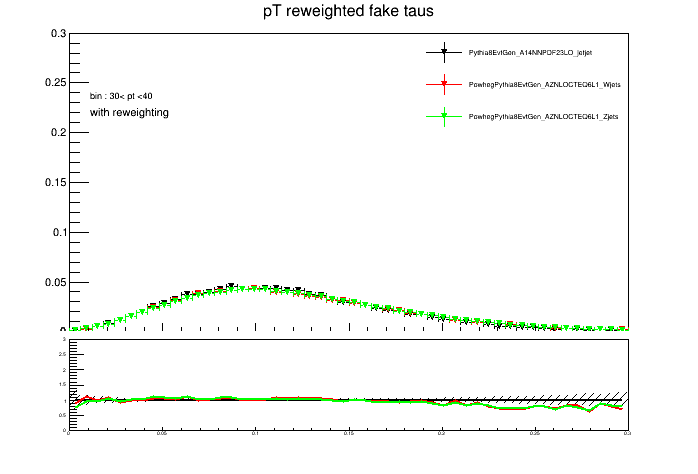
\includegraphics[width=0.35\textwidth]{FakeTau/AOD/MC16d/1p/gluon_Jet_Width_for_All_samples_and_in_bin_[30,40]_for_1_prong.png}}\hspace{0.05\textwidth}
\subbottom[]{\includegraphics[width=0.35\textwidth]{FakeTau/AOD/MC16d/3p/gluon_Jet_Width_for_All_samples_and_in_bin_[30,40]_for_3_prong.png}}\hspace{0.05\textwidth}
\subbottom[]{\includegraphics[width=0.35\textwidth]{FakeTau/AOD/MC16d/1p/gluon_Jet_Width_for_All_samples_and_in_bin_[40,60]_for_1_prong.png}}\hspace{0.05\textwidth}
\subbottom[]{\includegraphics[width=0.35\textwidth]{FakeTau/AOD/MC16d/3p/gluon_Jet_Width_for_All_samples_and_in_bin_[40,60]_for_3_prong.png}}\hspace{0.05\textwidth}
\subbottom[]{\includegraphics[width=0.35\textwidth]{FakeTau/AOD/MC16d/1p/gluon_Jet_Width_for_All_samples_and_in_bin_[60,90]_for_1_prong.png}}\hspace{0.05\textwidth}
\subbottom[]{\includegraphics[width=0.35\textwidth]{FakeTau/AOD/MC16d/3p/gluon_Jet_Width_for_All_samples_and_in_bin_[60,90]_for_3_prong.png}}\hspace{0.05\textwidth}
\subbottom[]{\includegraphics[width=0.35\textwidth]{FakeTau/AOD/MC16d/1p/gluon_Jet_Width_for_All_samples_and_in_bin_[90,150]_for_1_prong.png}}\hspace{0.05\textwidth}
\subbottom[]{\includegraphics[width=0.35\textwidth]{FakeTau/AOD/MC16d/3p/gluon_Jet_Width_for_All_samples_and_in_bin_[90,150]_for_3_prong.png}}\hspace{0.05\textwidth}
%\subbottom[]{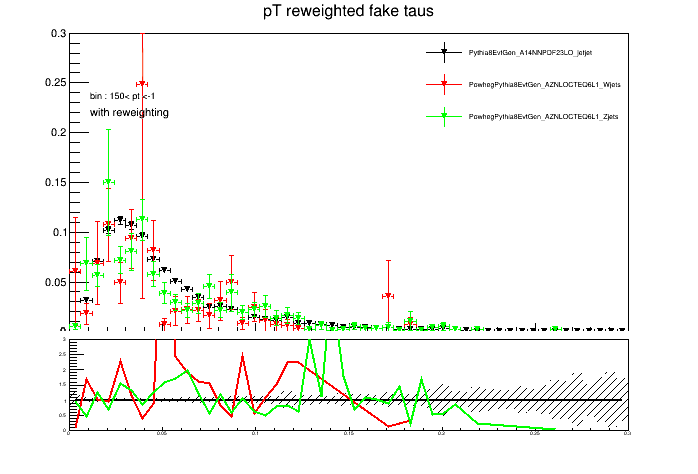
\includegraphics[width=0.35\textwidth]{FakeTau/AOD/MC16d/1p/gluon_Jet_Width_for_All_samples_and_in_bin_[150,-1]_for_1_prong.png}}\hspace{0.05\textwidth}
%\subbottom[]{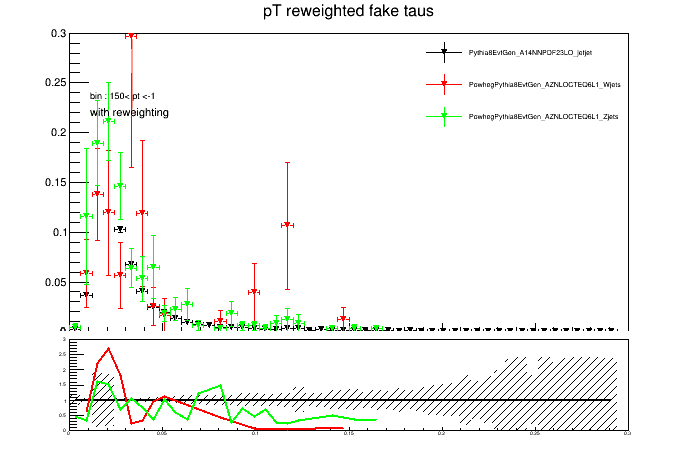
\includegraphics[width=0.35\textwidth]{FakeTau/AOD/MC16d/3p/gluon_Jet_Width_for_All_samples_and_in_bin_[150,-1]_for_3_prong.png}}\hspace{0.05\textwidth}
		\end{center}
		\caption{Jet Width templates of gluon tau-faking jets separated into \pt\ bins, going from top as the lowest \pt\ bin to bottom being the highest. Left column shows templates for 1 prong tau, while right columns shows 3 prong tau templates. Samples shown have been produced for the 2017 data collection period pile-up conditions.}
		\label{fig:2017_gluon_templates}
\end{figure}	

\begin{figure}[H]
	\begin{center}
\subbottom[]{\includegraphics[width=0.35\textwidth]{FakeTau/AOD/MC16d/1p/quark_Jet_Width_for_All_samples_and_in_bin_[20,30]_for_1_prong.png}}\hspace{0.05\textwidth}
\subbottom[]{\includegraphics[width=0.35\textwidth]{FakeTau/AOD/MC16d/3p/quark_Jet_Width_for_All_samples_and_in_bin_[20,30]_for_3_prong.png}}\hspace{0.05\textwidth}
\subbottom[]{\includegraphics[width=0.35\textwidth]{FakeTau/AOD/MC16d/1p/quark_Jet_Width_for_All_samples_and_in_bin_[30,40]_for_1_prong.png}}\hspace{0.05\textwidth}
\subbottom[]{\includegraphics[width=0.35\textwidth]{FakeTau/AOD/MC16d/3p/quark_Jet_Width_for_All_samples_and_in_bin_[30,40]_for_3_prong.png}}\hspace{0.05\textwidth}
\subbottom[]{\includegraphics[width=0.35\textwidth]{FakeTau/AOD/MC16d/1p/quark_Jet_Width_for_All_samples_and_in_bin_[40,60]_for_1_prong.png}}\hspace{0.05\textwidth}
\subbottom[]{\includegraphics[width=0.35\textwidth]{FakeTau/AOD/MC16d/3p/quark_Jet_Width_for_All_samples_and_in_bin_[40,60]_for_3_prong.png}}\hspace{0.05\textwidth}
\subbottom[]{\includegraphics[width=0.35\textwidth]{FakeTau/AOD/MC16d/1p/quark_Jet_Width_for_All_samples_and_in_bin_[60,90]_for_1_prong.png}}\hspace{0.05\textwidth}
\subbottom[]{\includegraphics[width=0.35\textwidth]{FakeTau/AOD/MC16d/3p/quark_Jet_Width_for_All_samples_and_in_bin_[60,90]_for_3_prong.png}}\hspace{0.05\textwidth}
\subbottom[]{\includegraphics[width=0.35\textwidth]{FakeTau/AOD/MC16d/1p/quark_Jet_Width_for_All_samples_and_in_bin_[90,150]_for_1_prong.png}}\hspace{0.05\textwidth}
\subbottom[]{\includegraphics[width=0.35\textwidth]{FakeTau/AOD/MC16d/3p/quark_Jet_Width_for_All_samples_and_in_bin_[90,150]_for_3_prong.png}}\hspace{0.05\textwidth}
%\subbottom[]{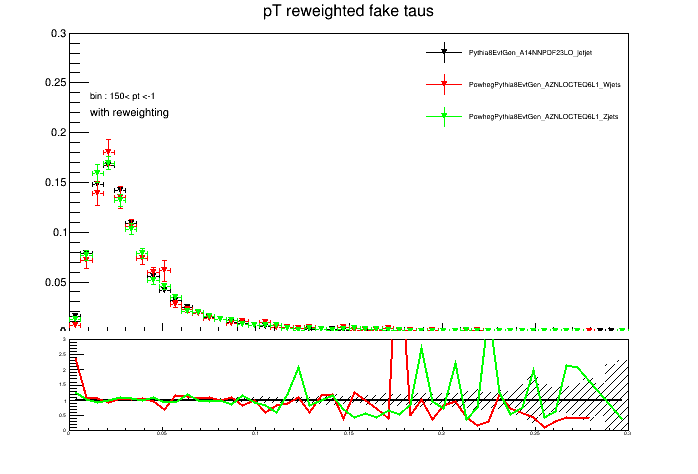
\includegraphics[width=0.35\textwidth]{FakeTau/AOD/MC16d/1p/quark_Jet_Width_for_All_samples_and_in_bin_[150,-1]_for_1_prong.png}}\hspace{0.05\textwidth}
%\subbottom[]{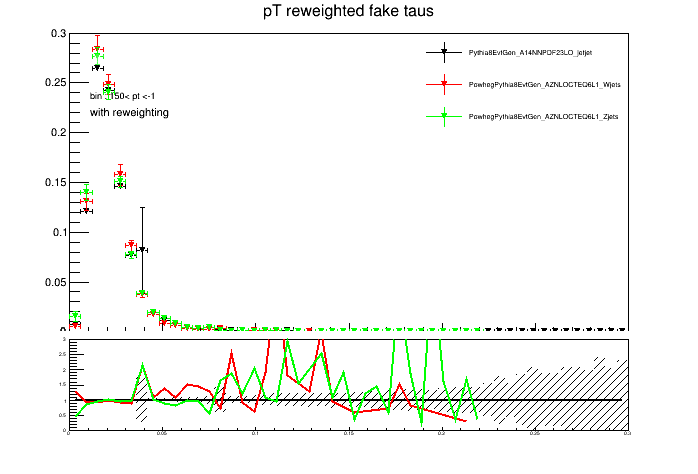
\includegraphics[width=0.35\textwidth]{FakeTau/AOD/MC16d/3p/quark_Jet_Width_for_All_samples_and_in_bin_[150,-1]_for_3_prong.png}}\hspace{0.05\textwidth}
		\end{center}
		\caption{Jet Width templates of quark tau-faking jets separated into \pt\ bins, going from top as the lowest \pt\ bin to bottom being the highest. Left column shows templates for 1 prong tau, while right columns shows 3 prong tau templates. Samples shown have been produced for the 2017 data collection period pile-up conditions.}
		\label{fig:2017_quark_templates}
\end{figure}	
